% !TEX root = main.tex

We evaluate the proposed nonparametric Gaussian mixture model based Thompson sampling (\ie \texttt{Nonparametric TS} as in Algorithm~\ref{alg:nonparametric_ts}) in diverse and complex synthetic datasets, for which practical methods that balance exploration and exploitation remain elusive.
Our goal is two-pronged:
\begin{enumerate}
	\item To compare the proposed \texttt{Nonparametric TS} algorithm to state-of-the-art alternatives (described in Section~\ref{ssec:ts_baselines}), showcasing its flexibility, generality and how it attains reduced regret in complex multi-armed bandits ---Section~\ref{ssec:evaluation_baselines}.
	\item To demonstrate that its performance is equivalent to an Oracle (\ie one that knows the true underlying model class) that implements a Thompson sampling policy ---Section~\ref{ssec:evaluation_oracle}.
\end{enumerate}

% State-of-the-art baselines
% !TEX root = main.tex
\subsection{Thompson sampling-based state-of-the-art baselines}
\label{ssec:ts_baselines}

Thompson sampling provides a bandit framework that requires access to posterior samples of the reward model.
An approach to extend its applicability to complex domains is to leverage the advances in Bayesian neural networks and to merge them with approximate Bayesian inference methods. The algorithms listed below are state-of-the art techniques that provide different computations of (or approximations to) reward posteriors that can be combined with Thompson sampling to address contextual multi-armed bandits.

\begin{enumerate}
	\item \texttt{LinearGaussian TS}: A powerful (not neural network based) Thompson sampling baseline, which assumes a contextual linear Gaussian reward function,
	\begin{equation}
	Y_{t,a}\sim \N{Y|x_t^\top\theta_a, \sigma_a^2} \;. \nonumber
	\end{equation}
	In its simplest setting, when the reward variance is known, the resulting Thompson sampling implementation follows that by~\citet{ip-Agrawal2013a}. In our experiments, in a similar fashion as done by~\citet{ip-Riquelme2018}, we model the joint distribution of $\theta_a$ and $\sigma_a^2$, $\forall a \in \A$, which allows the method to adaptively adjust to the observed reward noise. We leverage the Normal-inverse Gamma conjugate prior, \ie
	\begin{equation}
	\left(\theta_a, \sigma_a^2\right) \sim \NIG{\theta_a, \sigma_a^2 |m_{a,0}, \Sigma_{a,0},\alpha_{a,0}, \beta_{a,0}} \; ,
	\end{equation}
	of the Gaussian contextual model to derive the exact Bayesian posterior. We use an uninformative prior for the variance ($\alpha_{a,0}=1, \beta_{a,0}=1, \forall a$) and a standard uncorrelated Gaussian for the mean prior ($m_{a,0}=0, \Sigma_{a,0}=I, \forall a$).

	\item \texttt{MultitaskGP}: This is an alternative and popular Bayesian nonparametric technique that models context to reward mappings via Gaussian processes~\citep{ip-Srinivas2010,ip-Gruenewaelder2010,ic-Krause2011}. This implementation regresses the expected reward of different context-actions pairs by fitting a multitask Gaussian process given observed bandit data.
	
	\item \texttt{NeuralLinear}: This algorithm, introduced by~\citet{ip-Riquelme2018}, operates by learning a neural network that maps contexts to rewards for each action, and simultaneously, updates a Bayesian linear regression in the network's last layer. The last layer maps a learned representation $z$ linearly to the rewards $y$. The corresponding Thompson sampling draws the learned linear regression parameters $\theta_a$ for each arm, but keeps the representation $z$ output by the learned network. In our experiments, the representation network and the Bayesian linear posterior are retrained and updated at every MAB interaction.

	\item \texttt{NeuralBootstrapped}: This algorithm is based on~\citep{ic-Osband2016}, which trains simultaneously (in parallel) $Q$ neural networks based on different bootstrapped bandit histories $\HH_{1:t}^{(1)},\cdots, \HH_{1:t}^{(Q)}$. These are generated by adding each newly observed evidence $(x_{t}, a_{t}, y_{t})$ to each history $\HH_{1:t-1}^{(q)}$, $q=\{1, \cdots,Q\}$, independently and with probability $p \in (0, 1]$. In order to choose an action for a given context, one of the $q$ networks is selected with uniform probability ($1/Q$), and the best action according to the selected network is played.
	
	\item \texttt{NeuralRMS}: This is a simple bandit benchmark that trains a neural network to map contexts to rewards. At each time $t$, it acts $\epsilon$-greedily according to the current model, which due to the Stochastic Gradient Descent (SGD) algorithm used for training (\ie the RMSProp optimizer in this implementation), captures randomness in its output.
	
	\item \texttt{NeuralDropoutRMS}: Dropout is a neural network training technique where the output of each neuron is independently zeroed out with a given probability in each forward pass. Once the network is trained, dropout can also be used to obtain a distribution of predictions for a specific input. By choosing the best action with respect to the random dropout prediction, an implicit form of Thompson sampling is implemented.
	
	\item \texttt{NeuralParamNoise}: An approach to approximate a distribution over neural networks consists in randomly perturbing the point estimates attained by SGD on the available data~\cite{ip-Plappert2018}. In this case, the model uses a heuristic to control the amount of \iid noise it adds to the parameters of the neural network, which is used for making a decision, but not for training steps: SGD re-starts from the last, noiseless parameter value.
	
	\item \texttt{BNNVariationalGaussian}: This algorithm is based on ideas presented in~\citep{ip-Blundell2015} that combine stochastic variational inference and Bayes by backpropagation. It implements a Bayesian neural network by modeling each individual weight posterior as a univariate Gaussian distribution. Thompson sampling then draws a network at each time step by sampling each weight independently. The variational approach consists in maximizing a proxy for the maximum likelihood estimates of the network weights given observed data, to fit the unknown parameters of the variational posterior.
	
	\item \texttt{BNNAlphaDiv}: This technique leverages expecta\-tion\-/pro\-pagation and Black\-/box alpha\-/divergence minimization as in~\cite{ip-Hernandez-Lobato2016} to approximate the unknown reward distribution. The algorithm iteratively approximates the posterior of interest by updating a single approximation factor at a time, which usually corresponds to the likelihood of one data point. The implementation adopted here optimizes the global objective directly via stochastic gradient descent.
	
	\item \texttt{Optimal}: When possible (\ie for simulated bandits for which there is ground truth), we implement an optimal multi-armed bandit policy that selects the best arm for the given context, based on the known true expected reward of each arm.
\end{enumerate}

As reported by~\citet{ip-Riquelme2018}, deep learning methods are very sensitive to the selection of a wide variety of hyperparameters, and these hyperparameter choices are known to be highly dataset dependent. Besides, in bandit scenarios, we do not have access to each problem to perform any a-priori tuning. Therefore, we resort to the default settings provided by the authors in \href{https://github.com/tensorflow/models/tree/master/research/deep_contextual_bandits}{their implementation}.

A full description of these algorithms and all implementation details can be found in the \href{https://sites.google.com/site/deepbayesianbandits/}{original deep bandit showdown work}.
For completeness, we present the set of hyperparameters used for our experiments in Section~\ref{asec:evaluation_hyperparameters} of the Appendix. In addition, and following the insights from~\cite{ip-Riquelme2018} that partially optimized uncertainty estimates can lead to catastrophic decisions with neural networks, we retrain the neural network models at every iteration of the multi-armed bandit ---note that since stochastic gradient descent is used for training, randomness is incorporated in all implementations.



\subsection{Complex contextual bandits: reduced regret under model uncertainty}
\label{ssec:evaluation_baselines}

Our proposed nonparametric Thompson sampling is valuable for MAB scenarios in the presence of model uncertainty.
In the following, we show that \texttt{Nonparametric TS}, while avoiding case-by-case reward model design choices and bypassing model mispecification, attains reduced regret across a variety of bandit scenarios.

To that end, we evaluate its performance under different reward settings: in Section~\ref{sssec:evaluation_contextual_linear_baselines}, contextual linear Gaussian bandits~\footnote{Results for non-contextual Gaussian bandits are provided in Section~\ref{asec:noncontextual_gaussian_bandits} of the Appendix, showcasing how the proposed method attains satisfactory performance.}, and in Section~\ref{sssec:evaluation_mixture_scenarios_baselines} contextual bandits with rewards not in the exponential family.

% contextual linear Gaussian bandits
% !TEX root = main.tex
\subsubsection{Contextual linear Gaussian bandits}
\label{sssec:evaluation_contextual_linear_baselines}

We first investigate the performance of our proposed method in the classic contextual linear Gaussian MAB setting: \ie for bandits where rewards are drawn from linearly parameterized arms, where the mean reward for context $x_t$ and arm $a$ is given by $x_t^\top \theta_a$, for some unknown latent parameter $\theta_a$.

We evaluate different parameterizations of such bandits, both for non-sparse and sparse settings (where only few components of $\theta_a$ are non-zero for each arm).
Specifically, we draw a 10 dimensional $\theta_a$ uniformly at random (with only 3 components left as non-zero for each arm in the sparse setting), with contexts distributed as a 10-dimensional standard Gaussian. In all cases, Gaussian noise (with a minimum standard deviation of 0.01) is added to the rewards of each arm, for $|\mathcal{A}|=8$.

Figures~\ref{fig:linear_showdown_baselines_top_regret} and~\ref{fig:sparse_linear_showdown_baselines_top_regret} showcase the five top performing algorithms in non-sparse and sparse linear contextual bandits respectively, with cumulative regret results (and attained relative regret improvements) detailed in Tables~\ref{tab:linear_showdown_baselines_regret} and \ref{tab:sparse_linear_showdown_baselines_regret} for all the evaluated methods.
The corresponding reward results are provided in Section~\ref{asec:linearGaussian_baselines} of the Appendix.

% Linear Gaussian regret figure
\begin{figure}[!ht]
	\centering
	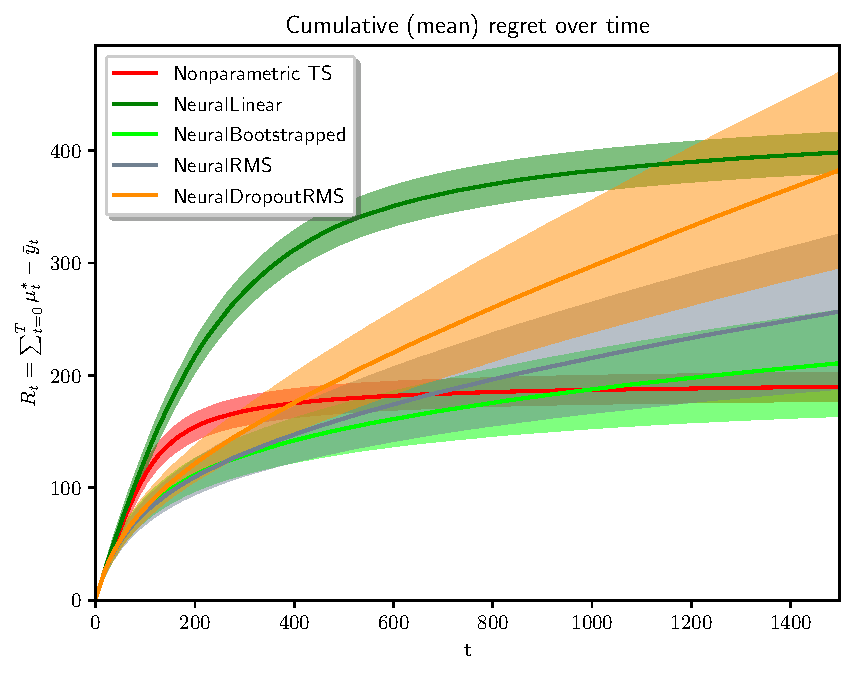
\includegraphics[width=0.75\textwidth]{./figs/linear_showdown_baselines/cum_optexpected_regret_top_five_std}
	\vspace*{-5ex}
	\caption{Mean regret (standard deviation shown as shaded region) for $R=500$ realizations of the presented methods in contextual linear Gaussian MABs.}
	\label{fig:linear_showdown_baselines_top_regret}
	\vspace*{-2ex}
\end{figure}
% Linear Gaussian regret figure
\begin{table}[!h]
	\caption{Cumulative regret at $t=1500$ for $R=500$ realizations of contextual linear Gaussian MABs. The second column showcases the additional relative cumulative regret incurred by each algorithm when compared to \texttt{Nonparametric TS} at $t=1500$.}
	\label{tab:linear_showdown_baselines_regret}
	\vspace*{-4ex}
	\begin{center}
		\resizebox*{0.75\textwidth}{!}{
			\begin{tabular}{|c|c|c|}
				\hline
				Algorithm 	\cellcolor[gray]{0.6} & Cumulative regret \cellcolor[gray]{0.6} & Relative cumulative regret \cellcolor[gray]{0.6} \\ \hline
				Nonparametric TS     	 & 189.889 & \%0.000 \\ \hline
				NeuralLinear         	 & 398.485 & \%109.852 \\ \hline
				NeuralBootstrapped   	 & 210.914 & \%11.073 \\ \hline
				NeuralRMS            	 & 256.897 & \%35.288 \\ \hline
				NeuralDropoutRMS     	 & 382.870 & \%101.629 \\ \hline
				NeuralParamNoise     	 & 241.039 & \%26.937 \\ \hline
				MultitaskGP          	 & 213.648 & \%12.512 \\ \hline
				BNNVariationalGaussian 	 & 827.369 & \%335.712 \\ \hline
				BNNAlphaDiv          	 & 793.118 & \%317.675 \\ \hline
			\end{tabular}
		}
	\end{center}
	\vspace*{-2ex}
\end{table}

We observe a reduced cumulative regret of our proposed nonparametric Thompson sampling when compared to all state-of-the-art Thompson sampling alternatives described in Section~\ref{ssec:ts_baselines}.
The proposed \texttt{Nonparametric TS} method achieves logarithmic regret, even as it estimates the true form of the underlying unknown reward function, resulting in considerably smaller regret than the alternatives ---designed to be flexible for complex bandit scenarios--- in the contextual linear Gaussian setting.

The neural network based linear Thompson sampling method (\ie \texttt{NeuralLinear}) achieves logarithmic regret as well, but suffers an important loss: an average cumulative regret that doubles that of \texttt{Nonparametric TS} at $t=1500$.

% Sparse Linear Gaussian regret figure
\begin{figure}[!ht]
	\vspace*{-2ex}
	\centering
	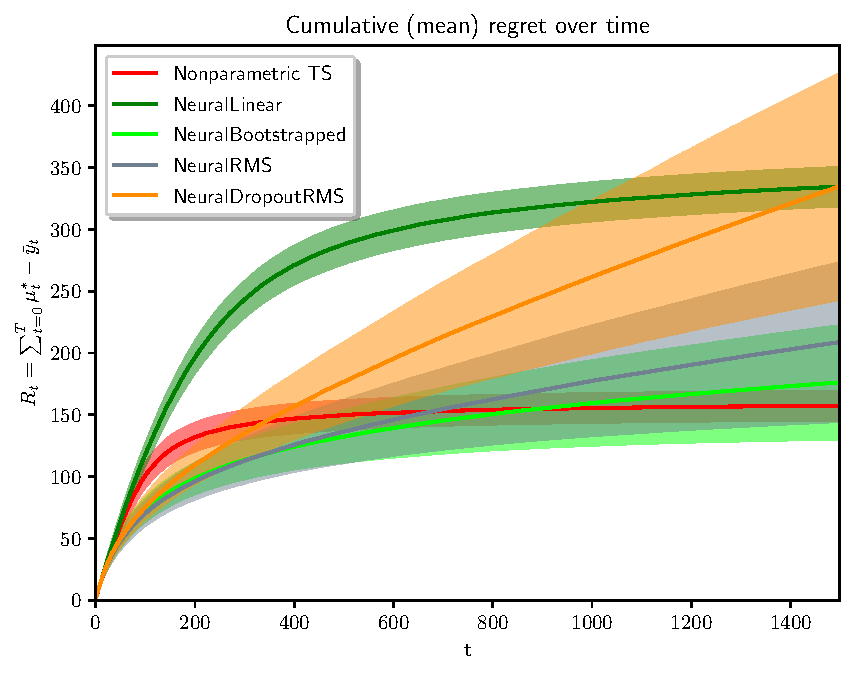
\includegraphics[width=0.75\textwidth]{./figs/sparse_linear_showdown_baselines/cum_optexpected_regret_top_five_std}
	\vspace*{-5ex}
	\caption{Mean regret (standard deviation shown as shaded region) for $R=500$ realizations of the presented methods in sparse contextual linear Gaussian MABs.}
	\label{fig:sparse_linear_showdown_baselines_top_regret}
	\vspace*{-2ex}
\end{figure}
% Sparse Linear Gaussian regret table
\begin{table}[!h]
	\caption{Cumulative regret at $t=1500$ for $R=500$ realizations of sparse contextual linear Gaussian MABs. The second column showcases the additional relative cumulative regret incurred by each algorithm when compared to \texttt{Nonparametric TS} at $t=1500$.}
	\label{tab:sparse_linear_showdown_baselines_regret}
	\vspace*{-4ex}
	\begin{center}
		\resizebox*{0.75\textwidth}{!}{
			\begin{tabular}{|c|c|c|}
				\hline
				Algorithm 	\cellcolor[gray]{0.6} & Cumulative regret \cellcolor[gray]{0.6} & Relative cumulative regret \cellcolor[gray]{0.6} \\ \hline
				Nonparametric TS     	 & 157.406 & \%0.000 \\ \hline
				NeuralLinear         	 & 334.569 & \%112.551 \\ \hline
				NeuralBootstrapped   	 & 176.136 & \%11.899 \\ \hline
				NeuralRMS            	 & 208.738 & \%32.611 \\ \hline
				NeuralDropoutRMS     	 & 334.870 & \%112.742 \\ \hline
				NeuralParamNoise     	 & 199.122 & \%26.502 \\ \hline
				MultitaskGP          	 & 186.023 & \%18.180 \\ \hline
				BNNVariationalGaussian 	 & 762.321 & \%384.301 \\ \hline
				BNNAlphaDiv          	 & 695.097 & \%341.594 \\ \hline
				
			\end{tabular}
		}
	\end{center}
	\vspace*{-2ex}
\end{table}

Bootstrapped and RMS based alternatives fail to achieve a good exploration-exploitation trade-off (their cumulative regret does not plateau by $t=1500$), with cumulative regrets that are at least 10\% and 30\% higher in all contextual MABs.
In addition, their performance is highly volatile across realizations of the same problem (recall their wide shaded regions in Figures~\ref{fig:linear_showdown_baselines_top_regret} and~\ref{fig:sparse_linear_showdown_baselines_top_regret}).
Specially concerning is the poor performance of all the Bayesian Neural Network (BNN) based baselines, which incur in more than \%300 cumulative regret increase with respect to \texttt{Nonparametric TS}.

These results support our claim that a nonparametric Bayesian based Thompson sampling is a flexible alternative that can provide reduced regret when compared to state-of-the-art baselines.

% Not-exponential contextual bandits
% !TEX root = main.tex
\subsubsection{Contextual bandits not in the exponential family}
\label{sssec:evaluation_mixture_scenarios_baselines}

We now study a set of more challenging contextual MABs, \ie those where the underlying reward distributions do not fit into the exponential family assumption.
Specifically, we study the following contextual bandit scenarios, where the context is randomly drawn from a two dimensional uniform distribution, \ie $x_{i,t}\sim\U{0,1}$, $i\in\{0,1\}$, $t\in \Natural$.

\texttt{Scenario A:}
\begin{equation}
\begin{cases}
p_{1}(y|x_t,\theta) = 0.5 \cdot \N{y|x_t^\top(0 \; 0), 1} + \; 0.5 \cdot \N{y|x_t^\top(1 \; 1), 1}\\
p_{2}(y|x_t,\theta) = 0.5 \cdot \N{y|x_t^\top(2 \; 2), 1} + \; 0.5 \cdot \N{y|x_t^\top(3 \; 3), 1}
\end{cases}
\nonumber
\end{equation}
\texttt{Scenario B:}
\begin{equation}
\begin{cases}
p_{1}(y|x_t,\theta) = 0.5 \cdot \N{y|x_t^\top(1 \; 1), 1} + \; 0.5 \cdot \N{y|x_t^\top(2 \; 2), 1}\\
p_{2}(y|x_t,\theta) = 0.3 \cdot \N{y|x_t^\top(0 \; 0), 1} + \; 0.7 \cdot \N{y|x_t^\top(3 \; 3), 1}
\end{cases}
\nonumber
\end{equation}
\texttt{Scenario C:}
\begin{equation}
\begin{cases}
p_{1}(y|x_t,\theta) = \N{y|x_t^\top(1 \; 1), 1}\; ,\\
p_{2}(y|x_t,\theta) = 0.5 \cdot \N{y|x_t^\top(1 \; 1), 1} + \; 0.5 \cdot \N{y|x_t^\top(2 \; 2), 1}\\
p_{3}(y|x_t,\theta) = 0.3 \cdot \N{y|x_t^\top(0 \; 0), 1} + \; 0.6 \cdot \N{y|x_t^\top(3 \; 3), 1} + \; 0.1 \cdot \N{y|x_t^\top(4 \; 4), 1} 
\end{cases}
\nonumber
\end{equation}
\texttt{Scenario D:}
\begin{equation}
\begin{cases}
p_{1}(y|x_t,\theta) = 0.75 \cdot \N{y|x_t^\top(0 \; 0), 1} + \; 0.25 \cdot \N{y|x_t^\top(0 \; 0), 10} \\
p_{2}(y|x_t,\theta) = 0.75 \cdot \N{y|x_t^\top(2 \; 2), 1} + \; 0.25 \cdot \N{y|x_t^\top(2 \; 2), 10}
\end{cases}
\nonumber
\end{equation}

The reward distributions of these contextual bandits are all Gaussian mixtures, which differ in the amount of mixture overlap and the similarity between arms.
In these scenarios, the reward functions are not within the exponential family of distributions: they are all multi-modal, unbalanced in \texttt{Scenarios B} and \texttt{C}, and with heavy tails in \texttt{Scenario D}.

\texttt{Scenario A} is a balanced mixture of two Gaussian distributions, with rewards easily separable per-arm.
On the contrary, there is a significant overlap between arm rewards in \texttt{Scenario B}, with quite unbalanced mixtures for arm 2: rewards from a mixand of low expected value are drawn with probability $0.3$, and higher rewards are expected with probability $0.7$.
\texttt{Scenario C} describes a MAB with different per-arm reward distributions: a linear Gaussian distribution for arm 1, a bi-modal Gaussian mixture for arm 2, and an unbalanced Gaussian mixture with three components for arm 3.
Finally, \texttt{Scenario D} models heavy-tailed distributions, where the bandit is subject to outlier rewards.

We show in Figure~\ref{fig:mixture_scenarios_bandit_showdown_baselines} how our proposed method adjusts to the underlying reward model complexity, attaining reduced cumulative regret when compared to other Thompson sampling-based alternatives, in all the studied scenarios.

% Mixture bandit regret figure (moved here so that it appears soon in text)
\begin{figure*}[!ht]
	\centering
	\begin{subfigure}[c]{0.45\textwidth}
		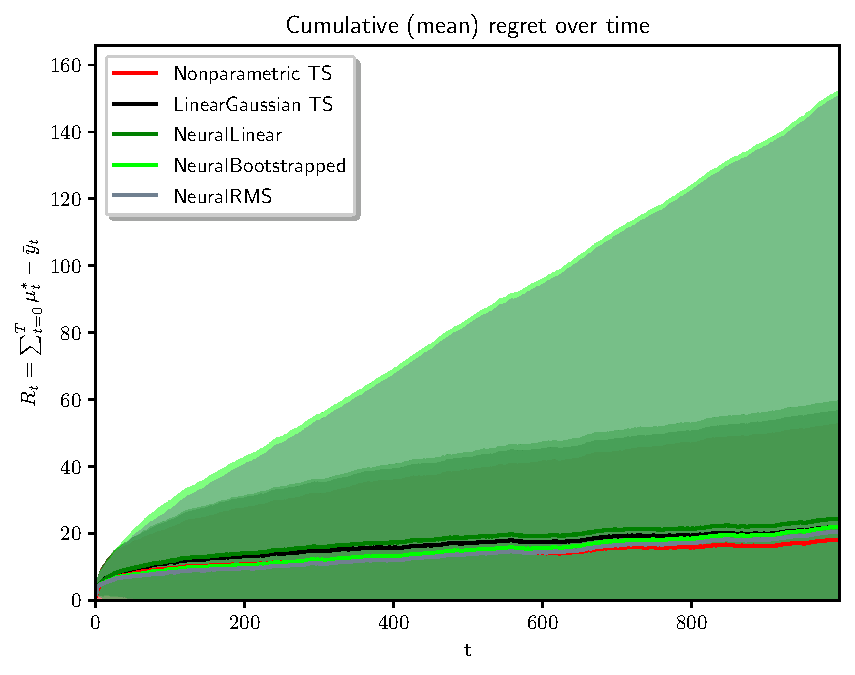
\includegraphics[width=\textwidth]{./figs/linear_gaussian_mixture_easy_baselines/cum_optexpected_regret_top_five_std}
		\vspace*{-5ex}
		\caption{\texttt{Scenario A}.}
		\label{fig:scenario_A_baselines_top}
	\end{subfigure}
	\begin{subfigure}[c]{0.45\textwidth}
		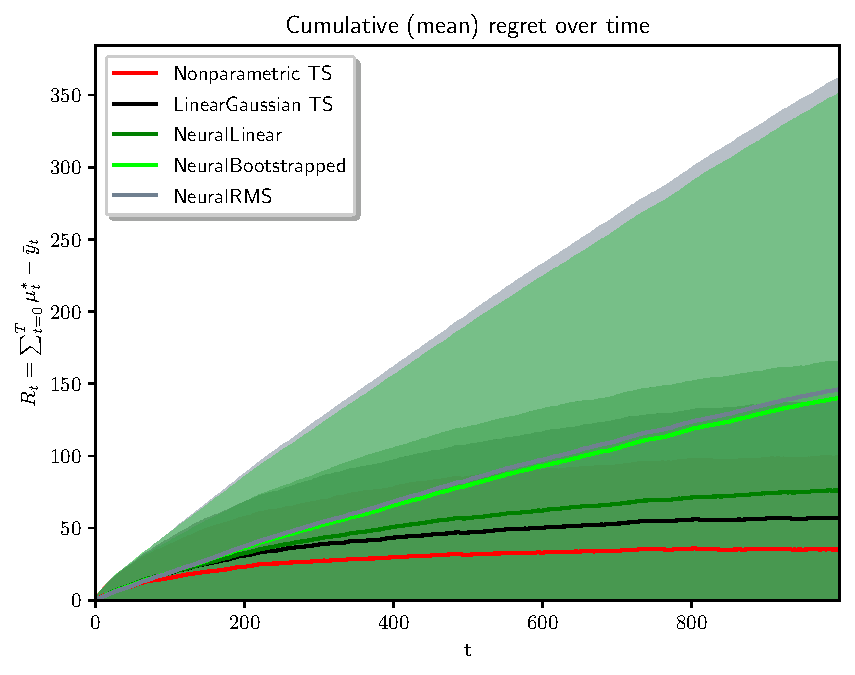
\includegraphics[width=\textwidth]{./figs/linear_gaussian_mixture_hard_baselines/cum_optexpected_regret_top_five_std}
		\vspace*{-5ex}
		\caption{\texttt{Scenario B}.}
		\label{fig:scenario_B_baselines_top}
	\end{subfigure}
	
	\begin{subfigure}[c]{0.45\textwidth}
		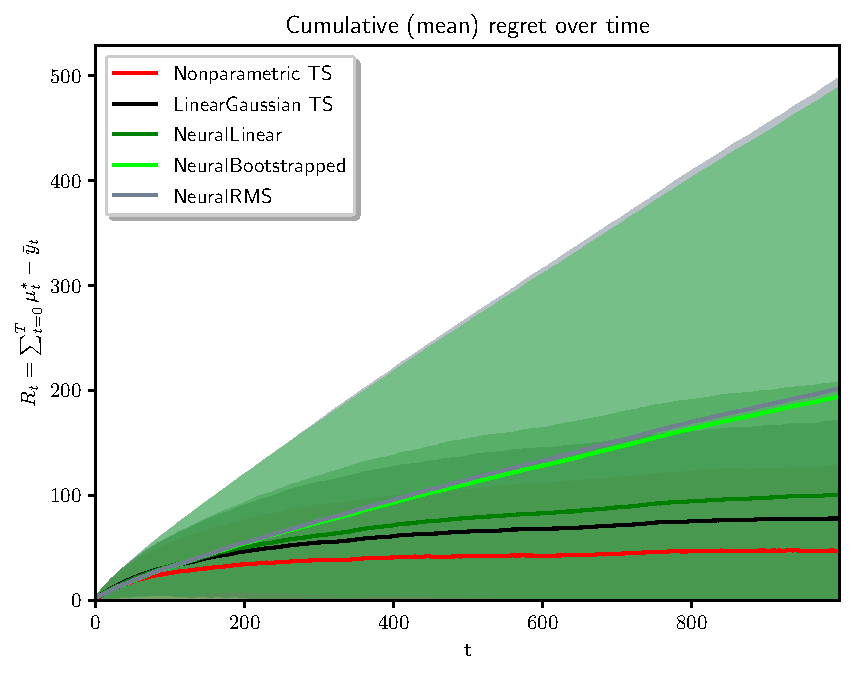
\includegraphics[width=\textwidth]{./figs/linear_gaussian_mixture_unbalanced_baselines/cum_optexpected_regret_top_five_std}
		\vspace*{-5ex}
		\caption{\texttt{Scenario C}.}
		\label{fig:scenario_C_baselines_top}
	\end{subfigure}
	\begin{subfigure}[c]{0.45\textwidth}
		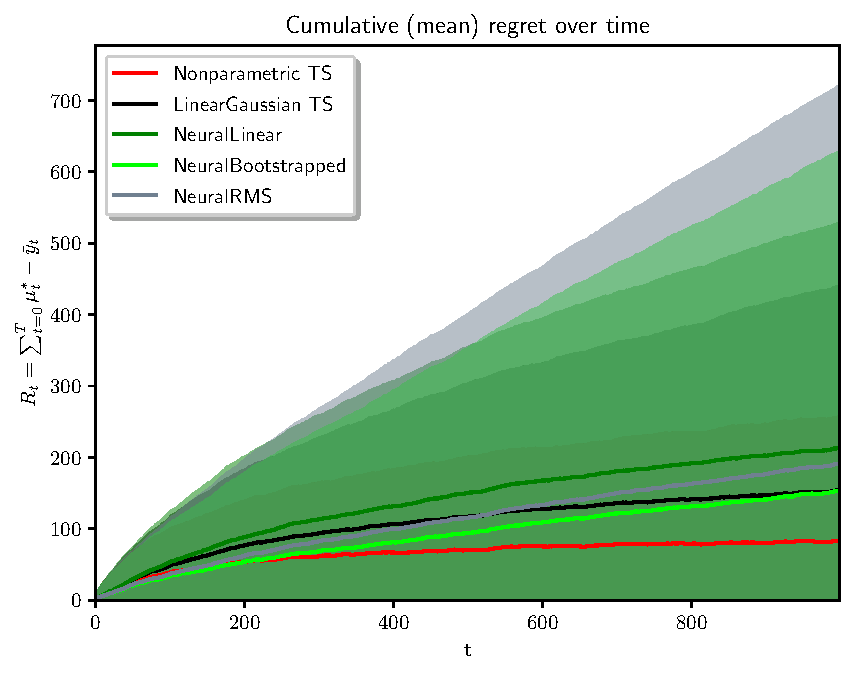
\includegraphics[width=\textwidth]{./figs/linear_gaussian_mixture_heavy_tail_baselines/cum_optexpected_regret_top_five_std}
		\vspace*{-5ex}
		\caption{\texttt{Scenario D}.}
		\label{fig:scenario_D_baselines_top}
	\end{subfigure}
	\vspace*{-2ex}
	\caption{Mean cumulative regret (standard deviation shown as shaded region) for $R=500$ realizations of the top-performing methods in all studied scenarios.}
	\label{fig:mixture_scenarios_bandit_showdown_baselines}
\end{figure*}

% Mixture bandit regret table
\begin{table*}[!ht]
	\caption{Mean cumulative regret at $t=1000$ for $R=500$ realizations of the studied methods in all scenarios. We indicate in parentheses the additional relative cumulative regret incurred by each algorithm when compared to \texttt{Nonparametric TS}.}
	\label{tab:mixture_scenarios_bandit_showdown_baselines_regret}
	\vspace*{-4ex}
	\begin{center}
		\resizebox*{\textwidth}{!}{
			\begin{tabular}{|c|c|c|c|c|}
				\hline
				Algorithm 	\cellcolor[gray]{0.6} & \texttt{Scenario A} \cellcolor[gray]{0.6} & \texttt{Scenario B} \cellcolor[gray]{0.6} & \texttt{Scenario C} \cellcolor[gray]{0.6} & \texttt{Scenario D} \cellcolor[gray]{0.6} \\ \hline
				Nonparametric TS       	& 18.105	 (\%0.000)	&	35.268	 (\%0.000)		&	47.172	 (\%0.000)		&	83.464	 (\%0.000) \\ \hline
				LinearGaussian TS      	& 21.957	 (\%21.276)	&	57.04	 (\%61.733)		&	77.921	 (\%65.184)		&	153.955	 (\%84.456) \\ \hline
				NeuralLinear           	& 24.358	 (\%34.538)	&	76.312	 (\%116.377)	&	100.202	 (\%112.415)	&	213.073	 (\%155.286) \\ \hline
				NeuralBootstrapped     	& 21.942	 (\%21.195)	&	140.302	 (\%297.816)	&	194.198	 (\%311.676)	&	153.315	 (\%83.690) \\ \hline
				NeuralRMS              	& 20.559	 (\%13.551)	&	146.276	 (\%314.756)	&	201.818	 (\%327.829)	&	191.552	 (\%129.501) \\ \hline
				NeuralDropoutRMS       	& 26.191	 (\%44.663)	&	146.182	 (\%314.490)	&	202.297	 (\%328.846)	&	170.3	 (\%104.039) \\ \hline
				NeuralParamNoise       	& 23.17	 	 (\%27.976)	&	129.758	 (\%267.921)	&	170.385	 (\%261.197)	&	177.931	 (\%113.182) \\ \hline
				MultitaskGP            	& 114.79	 (\%534.020)&	145.883	 (\%313.643)	&	245.441	 (\%420.305)	&	667.407	 (\%699.631) \\ \hline
				BNNVariationalGaussian  & 27.643	 (\%52.682)	&	172.461	 (\%389.001)	&	217.891	 (\%361.903)	&	340.92	 (\%308.462) \\ \hline
				BNNAlphaDiv            	& 67.969	 (\%275.416)&	196.028	 (\%455.824)	&	306.14	 (\%548.980)	&	247.998	 (\%197.130) \\ \hline
			\end{tabular}
		}
	\end{center}
	\vspace*{-4ex}
\end{table*}

In \texttt{Scenario A}, even if all shown methods attain logarithmic regret (\ie they are able to find the right exploitation-exploration balance) as shown in Figure~\ref{fig:scenario_A_baselines_top}, our proposed method attains meaningful regret reductions.
The attained cumulative regret results (with relative regret improvements) are detailed in Table~\ref{tab:mixture_scenarios_bandit_showdown_baselines_regret}, and the corresponding reward results are provided in Section~\ref{asec:mixture_baselines} of the Appendix.

In \texttt{Scenario A}, the second best performing \texttt{NeuralRMS} baseline incurs an additional 13.5\% cumulative regret when compared to \texttt{Nonparametric TS}, \texttt{LinearGaussian TS} is 21.3\% worse, and a regret increase of 21.2\% and 34.5\% is observed for the \texttt{NeuralBootstrapped} and \texttt{NeuralLinear} baselines, respectively.

\texttt{Nonparametric TS} provides important regret savings when compared to the best performing alternative in each scenario:
at least an additional 61.7\%, 65.2\% and 83.69\% cumulative regret is incurred by other baselines at the end of \texttt{Scenario B}, \texttt{Scenario C}, and \texttt{Scenario D}, respectively.
The proposed Bayesian nonparametric mixture model Thompson sampling clearly outperforms all the alternatives in the studied scenarios.
Besides, the volatility in regret performance of \texttt{Nonparametric TS} is the smallest of all the studied alternatives across all scenarios.

Even if each scenario is a different MAB setting, \texttt{Nonparametric TS} is readily applicable to all, without any per-case specific fine-tuning:
even in \texttt{Scenario C}, where there are different model classes per-arm.
Overall, \texttt{Nonparametric TS} attains reduced regret in all the studied MABs ---with different unknown per-arm distributions not in the exponential family.

On the contrary, we observe a poor performance of neural network and approximate Bayesian inference based alternatives.
Specifically, we find that the linear neural alternative takes longer to reach the exploration-exploitation tradeoff.
\citet{ip-Riquelme2018} argued that \texttt{NeuralLinear} is able to simultaneously learn a good latent data representation, and to accurately quantify the uncertainty over linear models, to explain the observed rewards in terms of these learned representation. This competitive advantage allowed~\citet{ip-Riquelme2018} to successfully solve problems that require non-linear representations where linear approaches fail. However, we here observe a significant regret increase in comparison to our proposed nonparametric method for bandits with reward functions not in the exponential family:
additional 34.54\%, 116.377\%, 112.415\% and 155.29\% regret is incurred in \texttt{Scenarios A}, \texttt{B}, \texttt{C}, and \texttt{D}, respectively.

In addition, bootstrapped and RMS based neural Thompson sampling techniques struggle to find a good exploration-exploitation balance, incurring in additional (and very volatile) regret performance, as shown in Figure~\ref{fig:mixture_scenarios_bandit_showdown_baselines}.
As noted by~\citet{ip-Riquelme2018}, ($i$) bootstrapping incurs in a heavy computational overhead, depending on the number of networks considered; ($ii$) a noise-injection based method is hard to tune and sensitive to the heuristic controlling the injected noise-level; and ($iii$) dropout algorithms heavily depend on their hyperparameters, and it is unclear how to disentangle better training from better exploration in these models. On the contrary, \texttt{Nonparametric TS} achieves reduced regret across all scenarios without any case-specific fine-tuning.

Alternative nonparametric methods, such as those based on Gaussian processes also suffer in all the studied scenarios (see Table~\ref{tab:mixture_scenarios_bandit_showdown_baselines_regret}). We argue that the low performance of this method is explained by model misspecification: Gaussian process regression methods require knowledge of the true underlying model class (\ie what mean and kernel functions to use) ---if the reward model class of the MAB they are targeting is not correctly specified, then increased regret is attained. Note that, in \texttt{Nonparametric TS}, no per-MAB fine tuning is required.

Variational inference and expectation-propagation based algorithms also perform poorly in all the studied scenarios (see Table~\ref{tab:mixture_scenarios_bandit_showdown_baselines_regret}). As reported by~\citet{ip-Riquelme2018}, while optimizing to convergence at every interaction with the world incurs increased computational cost, results suggest that it may not be sufficient to partially optimize the variational parameters in bandit settings. Similarly, for Black-Box $\alpha$-divergence, partial convergence may be the cause of poor performance. Overall, there is a need for investigating how to sidestep the slow convergence of the uncertainty estimates in bandit settings for these neural network based methods.

The volatility of all the evaluated neural network based alternatives is noteworthy, and worrisome: their performance is highly variable when compared to the proposed nonparametric method (reward standard deviation details are provided in Section~\ref{asec:mixture_baselines} of the Appendix.).

On the contrary, the performance of \texttt{Nonparametric TS} is much less volatile.
For real-life bandit applications, the variance of an algorithm's performance is critical: even if expected reward guarantees are in place, the understanding of how volatile a bandit algorithm's decisions are, has undeniable real-world impact.

All in all, we conclude that our proposed nonparametric Thompson sampling outperforms (both in averaged cumulative regret, and in regret volatility) other alternatives across all the studied scenarios. Due to the capacity of Bayesian nonparametrics to autonomously adjust the complexity of the model to the sequentially observed data, the proposed method can, without any per-scenario tuning ($Gibbs_{max}=10$, $d_a=0$, $\gamma_a=0.1$, $\forall a$, in all the experiments), readily target all of them, and attain considerable regret reductions.

Important savings are achieved for MAB settings not in the exponential family (\ie unbalanced and heavy tailed distributions) and for bandits with different per-arm reward distributions, where we observe that alternative methods struggle.
The competitive advantage lies on the capacity of Bayesian nonparametrics to adjust the complexity of the posterior density to the sequentially observed bandit data. 

% Gibbs
\begin{figure*}[!h]
	\centering
	\begin{subfigure}[c]{0.45\textwidth}
		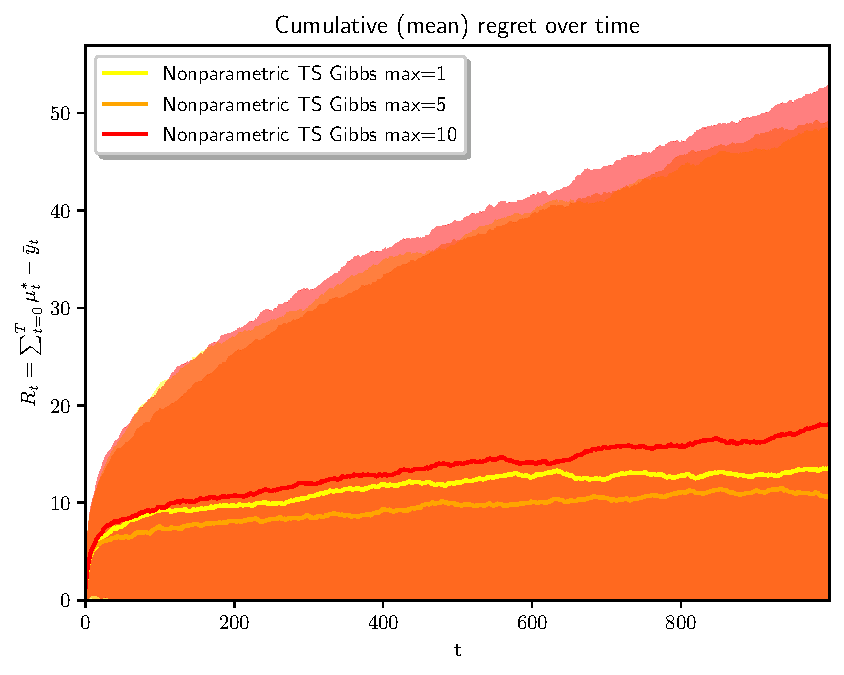
\includegraphics[width=\textwidth]{./figs/linear_gaussian_mixture_easy_gibbsmaxiter/cum_optexpected_regret_top_five_std}
		\vspace*{-5ex}
		\caption{\texttt{Scenario A}.}
		\label{fig:scenario_A_gibbsmaxiter_std}
	\end{subfigure}
	\begin{subfigure}[c]{0.45\textwidth}
		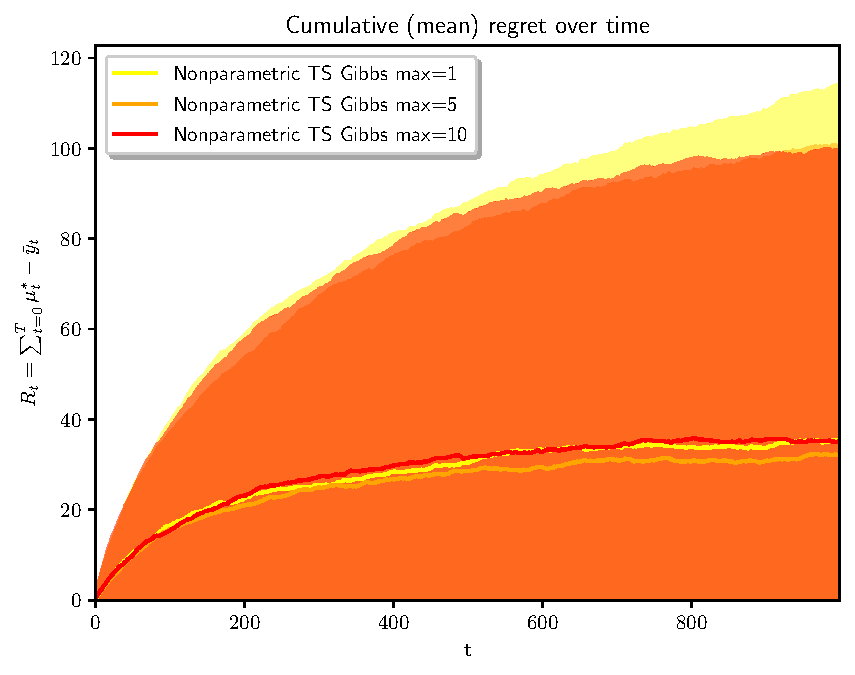
\includegraphics[width=\textwidth]{./figs/linear_gaussian_mixture_hard_gibbsmaxiter/cum_optexpected_regret_top_five_std}
		\vspace*{-5ex}
		\caption{\texttt{Scenario B}.}
		\label{fig:scenario_B_gibbsmaxiter_std}
	\end{subfigure}
	
	\begin{subfigure}[c]{0.45\textwidth}
		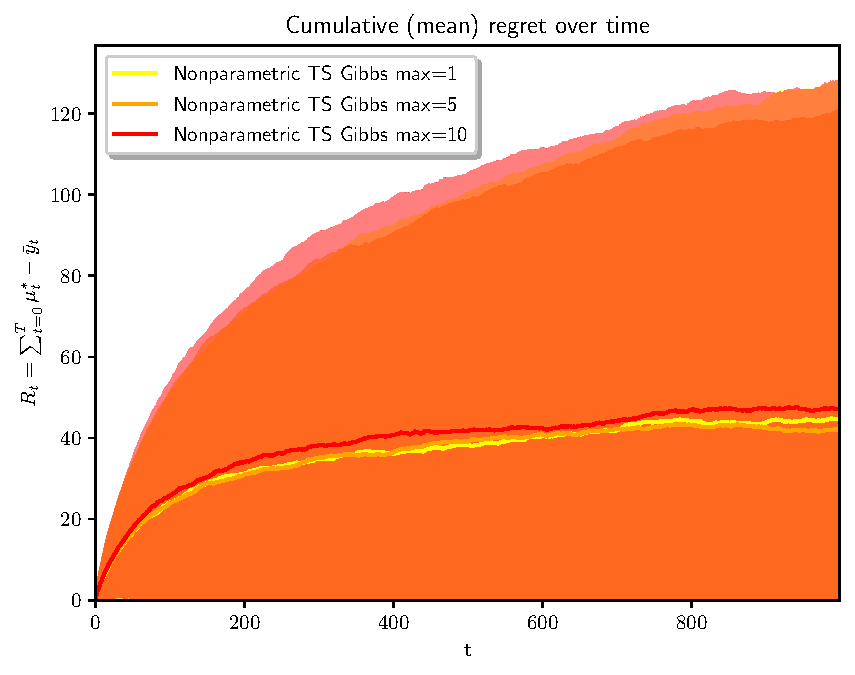
\includegraphics[width=\textwidth]{./figs/linear_gaussian_mixture_unbalanced_gibbsmaxiter/cum_optexpected_regret_top_five_std}
		\vspace*{-5ex}
		\caption{\texttt{Scenario C}.}
		\label{fig:scenario_C_gibbsmaxiter_std}
	\end{subfigure}
	\begin{subfigure}[c]{0.45\textwidth}
		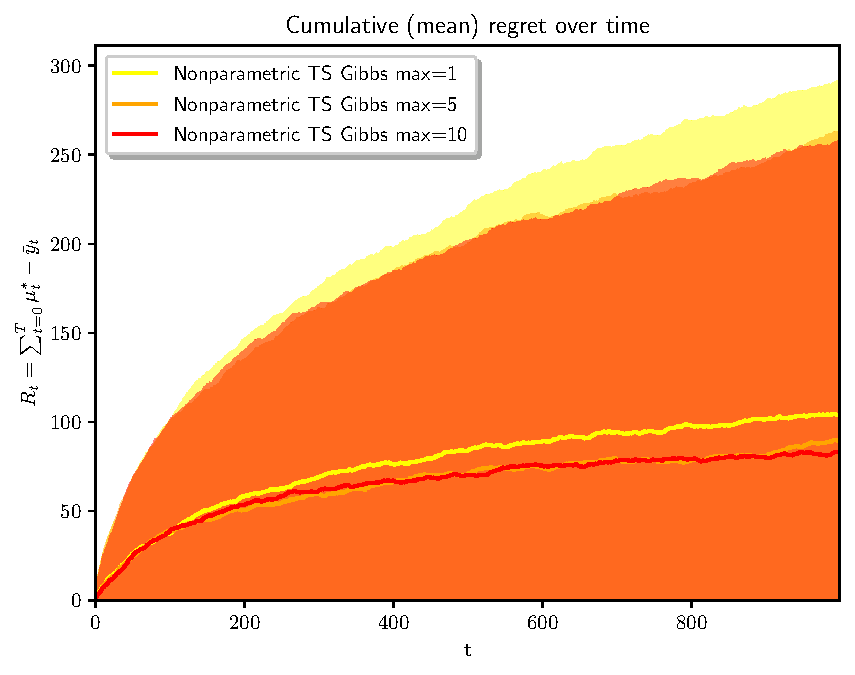
\includegraphics[width=\textwidth]{./figs/linear_gaussian_mixture_heavy_tail_gibbsmaxiter/cum_optexpected_regret_top_five_std}
		\vspace*{-5ex}
		\caption{\texttt{Scenario D}.}
		\label{fig:scenario_D_gibbsmaxiter_std}
	\end{subfigure}
	\vspace*{-2ex}
	\caption{Mean regret (standard deviation shown as shaded region) for $R=500$ realizations of the proposed \texttt{Nonparametric TS} method with different $Gibbs_{max}$ in all scenarios.}
	\label{fig:mixture_scenarios_bandit_showdown_gibbsmaxiter}
\end{figure*}

Finally, we investigate the \textit{warm-start} effect in the proposed algorithm's Gibbs sampling procedure, and how the practical recommendations on limiting the number of Gibbs iterations of Section~\ref{sssec:nonparametric_thompson_sampling_computational_complexity} impact regret performance.

In general, and because of the incremental availability of observations in the bandit setting, we observe that the proposed Gibbs sampler achieves quick convergence: in all our experiments, a 1\% log-likelihood relative difference between iterations is usually achieved within $Gibbs_{max}\leq10$ iterations.
We show in Figure~\ref{fig:mixture_scenarios_bandit_showdown_gibbsmaxiter} that no significant regret performance improvement is achieved by letting the sampler run for a high number of iterations. 

\textit{A good enough} posterior convergence at a limited computational budget ---at most $Gibbs_{max}$ updates over all $t_a$ observations for the played arm--- is possible because the Gibbs sampler is run, at each interaction with the world, from a good starting point: the per-arm parameter space that describes all but this newly observed reward.

Therefore, when computational constraints are appropriate, \eg for real-time bandits, limiting the number of Gibbs iterations allows for a drastic reduction in execution-time (see run-time details in Section~\ref{asec:exec_times} of the appendix), yet still achieving satisfactory cumulative regret.


\subsection{Nonparametric TS compared to Oracle TS}
\label{ssec:evaluation_oracle}

In the previous section, we showed that the proposed \texttt{Nonparametric TS} outperforms state-of-the-art Thompson sampling alternatives.
Our aim now is to determine how optimal the proposed nonparametric Bayesian based technique is.

To fully reveal the flexibility the proposed method, we scrutinize the \texttt{Nonparametric TS} algorithm by comparing it to \texttt{Oracle TS} algorithms: \ie Oracles that know the true per-arm reward distributions of the bandit they are targeted to.

This is an unrealistic setting in practice, yet possible in a simulated environment, as knowing the reward complexity of a MAB beforehand is impractical~\footnote{An alternative would be to run multiple model assumptions in parallel, with a subsequent model selection.}.

We implement \texttt{Oracle TS} algorithms for each simulated contextual bandit setting. Results below demonstrate how, due to the flexible and general density estimation technique provided by Bayesian nonparametric models, the per-arm nonparametric posterior densities converge to the true unknown distribution, allowing for our \texttt{Nonparametric TS} method to incur in minimal additional regret when compared to \texttt{Oracle TS} alternatives in all the studied scenarios.

% contextual linear Gaussian bandits
% !TEX root = main.tex
\subsubsection{Contextual linear Gaussian bandits: Oracle TS}
\label{sssec:evaluation_contextual_linear_oracle}

% Linear Gaussian results (moved to place them here)
\begin{figure*}[!h]
	% A=2
	\centering
	\begin{subfigure}[b]{0.32\textwidth}
		\centering
		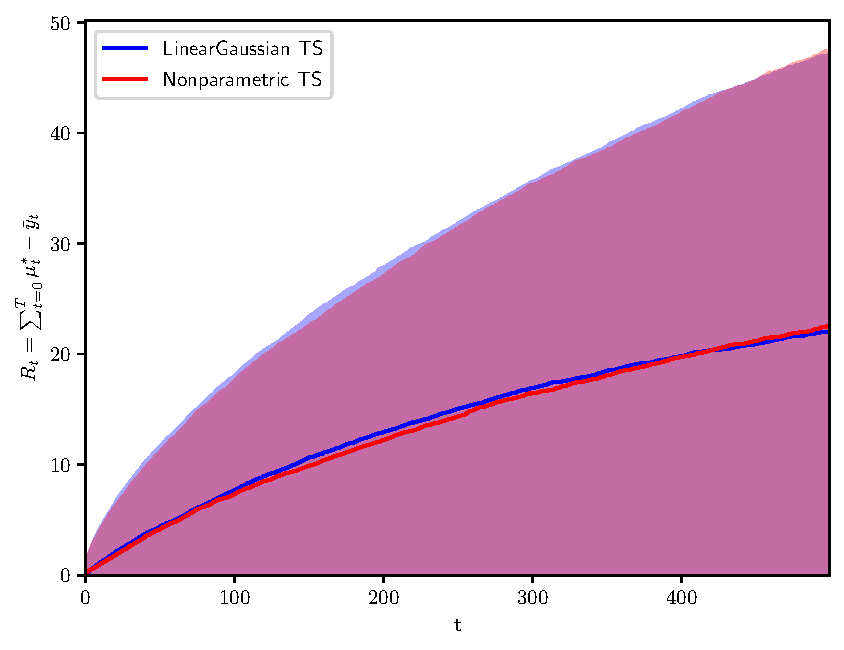
\includegraphics[width=\textwidth]{./figs/linearGaussian/cumregret_A2_-01_-01_01_01_1_1}
		\vspace*{-5ex}
		\caption{$|\mathcal{A}|=2$,\\ \hspace*{0.3cm} $\theta_{0,i}=-0.1$, $\theta_{1,i}=0.1$.}
		\label{fig:linear_gaussian_A2_01}
	\end{subfigure}
	\begin{subfigure}[b]{0.32\textwidth}
		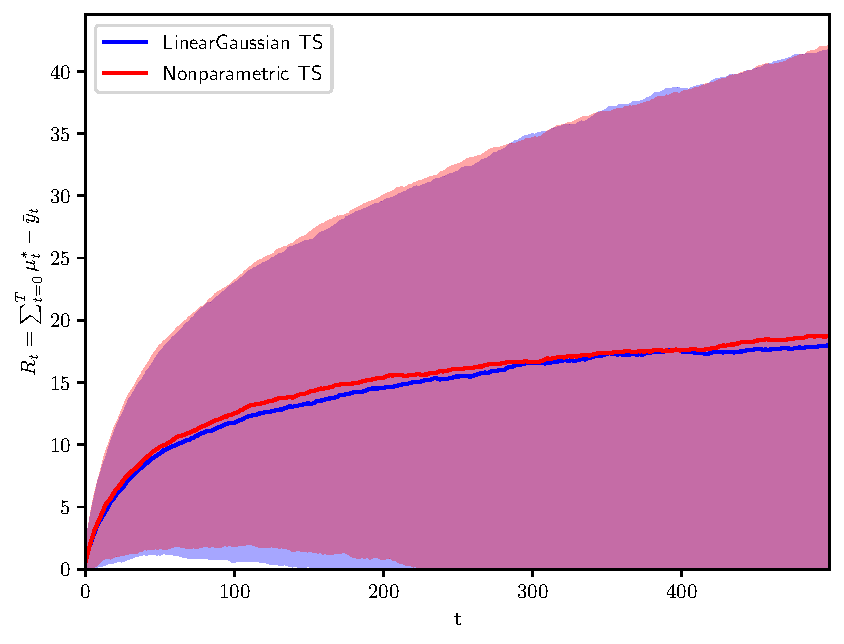
\includegraphics[width=\textwidth]{./figs/linearGaussian/cumregret_A2_-05_-05_05_05_1_1}
		\vspace*{-5ex}
		\caption{$|\mathcal{A}|=2$,\\ \hspace*{0.3cm}  $\theta_{0,i}=-0.5$, $\theta_{1,i}=0.5$.}
		\label{fig:linear_gaussian_A2_05}
	\end{subfigure}
	\begin{subfigure}[b]{0.32\textwidth}
		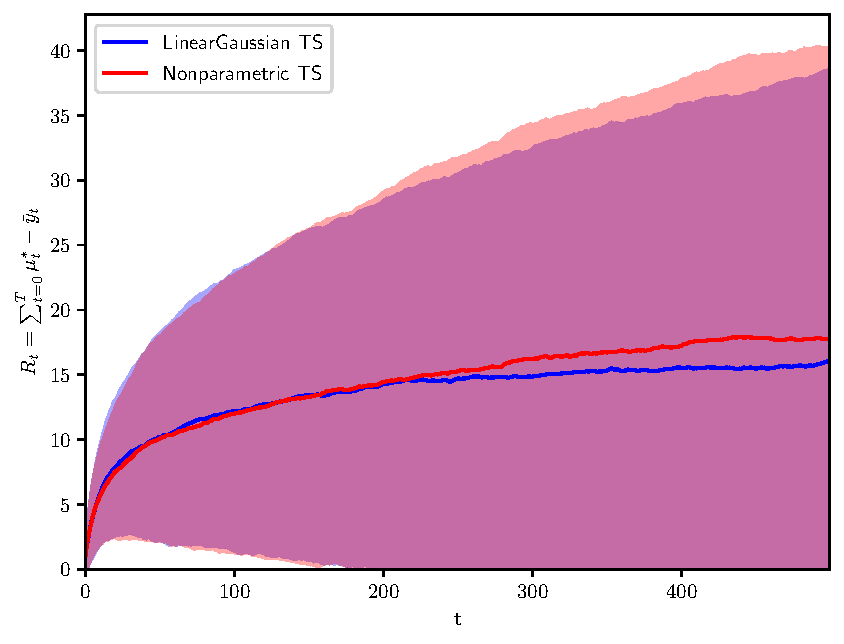
\includegraphics[width=\textwidth]{./figs/linearGaussian/cumregret_A2_-1_-1_1_1_1_1}
		\vspace*{-5ex}
		\caption{$|\mathcal{A}|=2$,\\ \hspace*{0.3cm}  $\theta_{0,i}=-1$, $\theta_{1,i}=1.0$.}
		\label{fig:linear_gaussian_A2_1}
	\end{subfigure}
	
	% A=3
	\begin{subfigure}[b]{0.32\textwidth}
		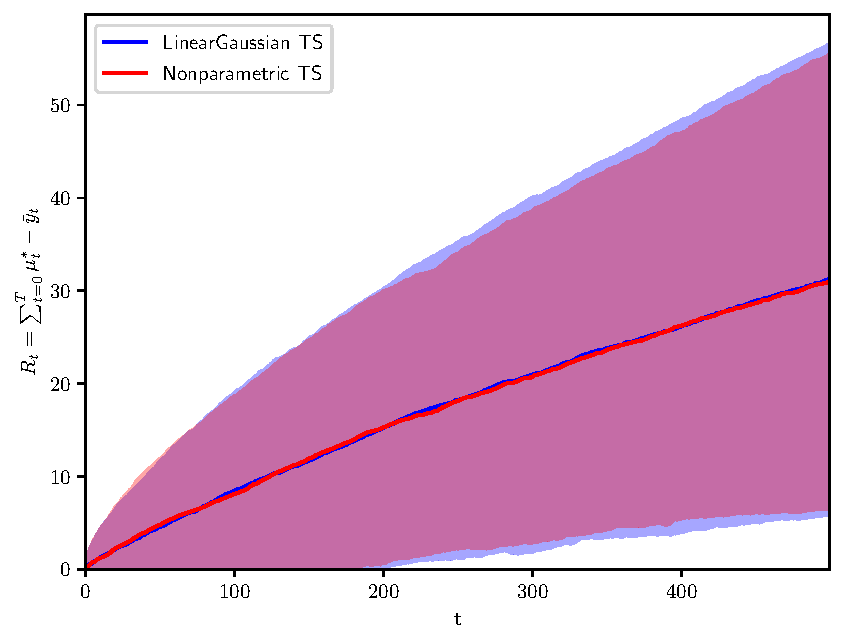
\includegraphics[width=\textwidth]{./figs/linearGaussian/cumregret_A3_-01_-01_0_0_01_01_1_1_1}
		\vspace*{-5ex}
		\caption{$|\mathcal{A}|=3, \theta_{0,i}=-0.1$, \\ \hspace*{0.3cm}$\theta_{0,i}=0, \theta_{2,i}=0.1$.}
		\label{fig:linear_gaussian_A3_01}
	\end{subfigure}
	\begin{subfigure}[b]{0.32\textwidth}
		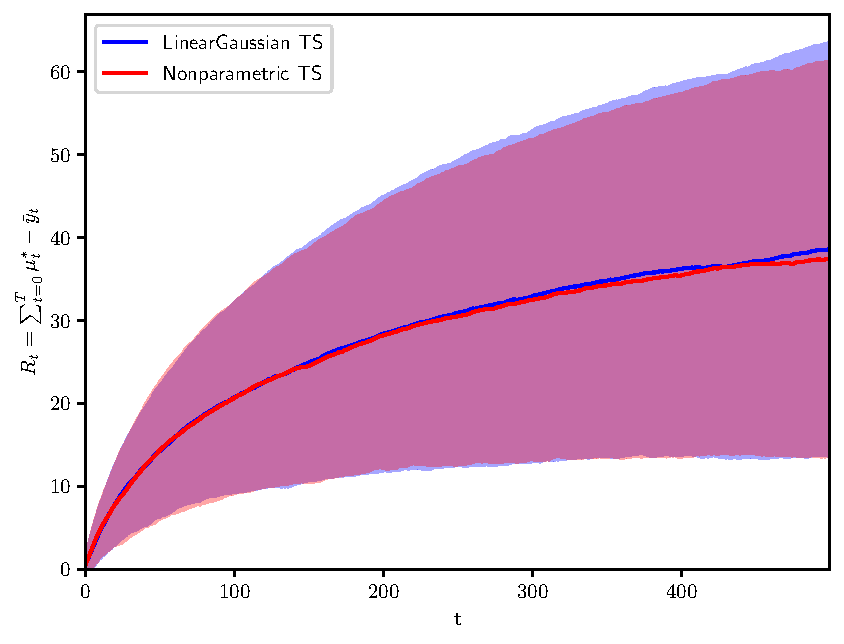
\includegraphics[width=\textwidth]{./figs/linearGaussian/cumregret_A3_-05_-05_0_0_05_05_1_1_1}
		\vspace*{-5ex}
		\caption{$|\mathcal{A}|=3, \theta_{0,i}=-0.5$, \\ \hspace*{0.3cm}$\theta_{1,i}=0, \theta_{2,i}=0.5$.}
		\label{fig:linear_gaussian_A3_05}
	\end{subfigure}
	\begin{subfigure}[b]{0.32\textwidth}
		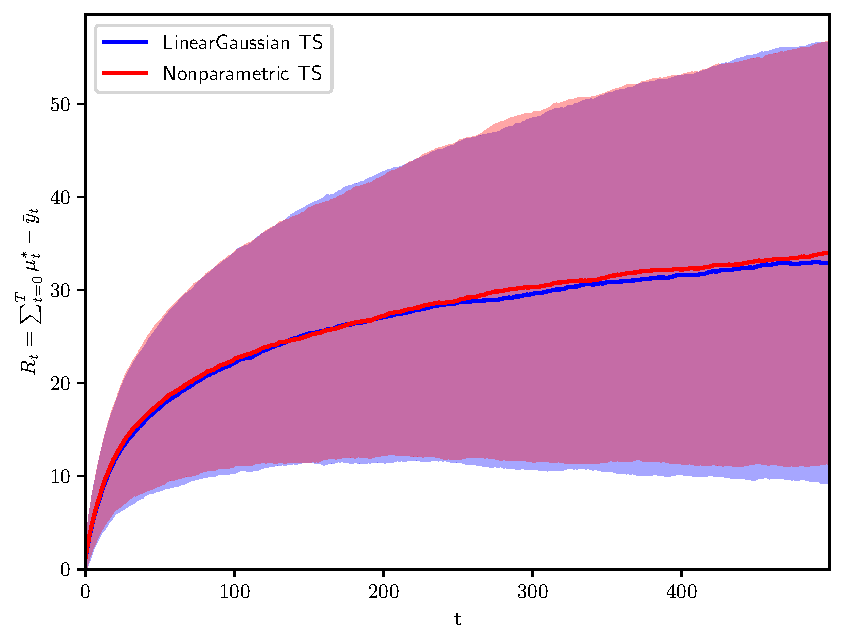
\includegraphics[width=\textwidth]{./figs/linearGaussian/cumregret_A3_-1_-1_0_0_1_1_1_1_1}
		\vspace*{-5ex}
		\caption{$|\mathcal{A}|=3, \theta_{0,i}=1$, \\ \hspace*{0.3cm}$\theta_{1,i}=0, \theta_{2,i}=1$.}
		\label{fig:linear_gaussian_A3_1}
	\end{subfigure}
	
	% A=4
	\begin{subfigure}[b]{0.32\textwidth}
		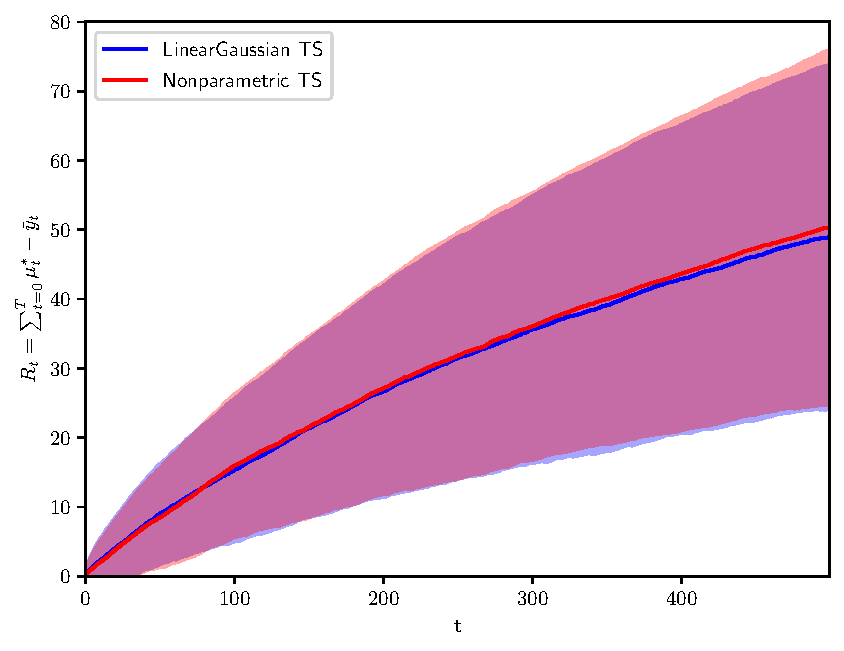
\includegraphics[width=\textwidth]{./figs/linearGaussian/cumregret_A4_-02_-02_-01_-01_01_01_02_02_1_1_1_1}
		\vspace*{-5ex}
		\caption{$|\mathcal{A}|=4, \theta_{0,i}=-0.2$,\\ \hspace*{0.3cm} $\theta_{1,i}=-0.1, \theta_{2,i}=0.1$,\\ \hspace*{0.3cm} $\theta_{3,i}=0.1$.}
		\label{fig:linear_gaussian_A4_01}
	\end{subfigure}
	\begin{subfigure}[b]{0.32\textwidth}
		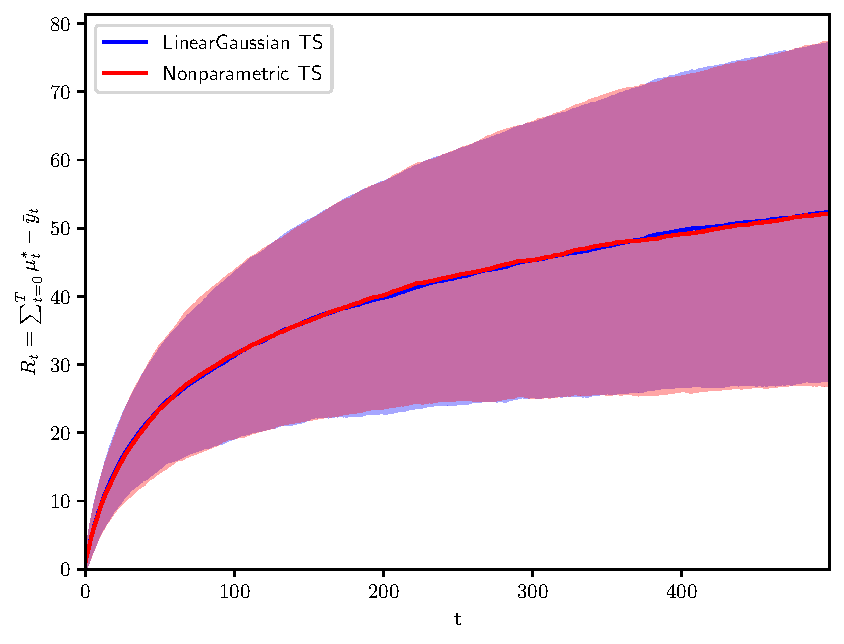
\includegraphics[width=\textwidth]{./figs/linearGaussian/cumregret_A4_-1_-1_-05_-05_05_05_1_1_1_1_1_1}
		\vspace*{-5ex}
		\caption{$|\mathcal{A}|=4, \theta_{0,i}=-1$,\\ \hspace*{0.3cm} $\theta_{1,i}=-0.5, \theta_{2,i}=0.5$,\\ \hspace*{0.3cm} $\theta_{3,i}=1$.}
		\label{fig:linear_gaussian_A4_05}
	\end{subfigure}
	\begin{subfigure}[b]{0.32\textwidth}
		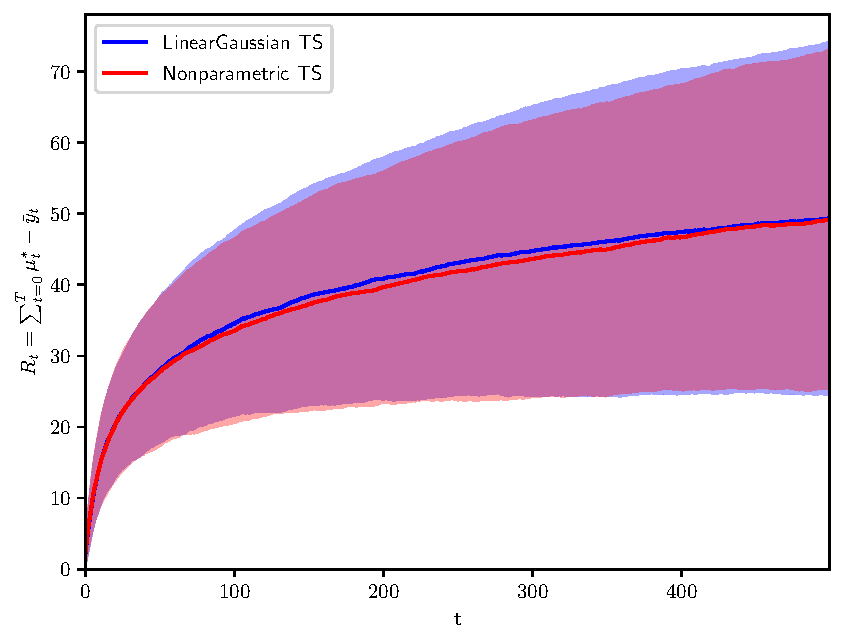
\includegraphics[width=\textwidth]{./figs/linearGaussian/cumregret_A4_-2_-2_-1_-1_1_1_2_2_1_1_1_1}
		\vspace*{-5ex}
		\caption{$|\mathcal{A}|=4, \theta_{0,i}=-2$,\\ \hspace*{0.3cm} $\theta_{1,i}=-1, \theta_{2,i}=1$,\\ \hspace*{0.3cm} $\theta_{3,i}=2$.}
		\label{fig:linear_gaussian_A4_1}
	\end{subfigure}
	
	\begin{subfigure}[b]{0.32\textwidth}
		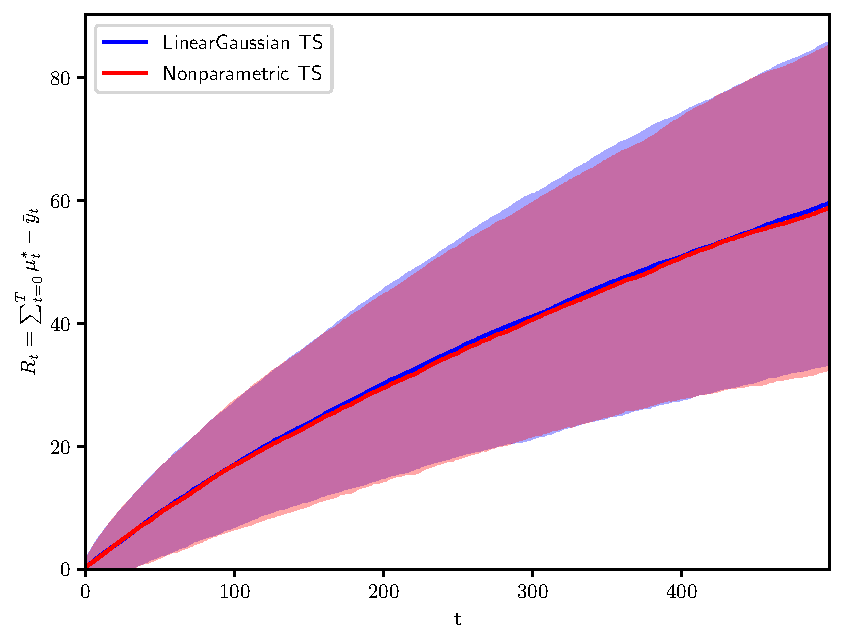
\includegraphics[width=\textwidth]{./figs/linearGaussian/cumregret_A5_-02_-02_-01_-01_0_0_01_01_02_02_1_1_1_1_1}
		\vspace*{-5ex}
		\caption{$|\mathcal{A}|=5, \theta_{0,i}=-0.2$,\\ \hspace*{0.3cm} $\theta_{1,i}=-0.1$, $\theta_{2,i}=0$,\\ \hspace*{0.3cm} $\theta_{3,i}=0.1, \theta_{4,i}=0.1$.}
		\label{fig:linear_gaussian_A5_01}
	\end{subfigure}
	\begin{subfigure}[b]{0.32\textwidth}
		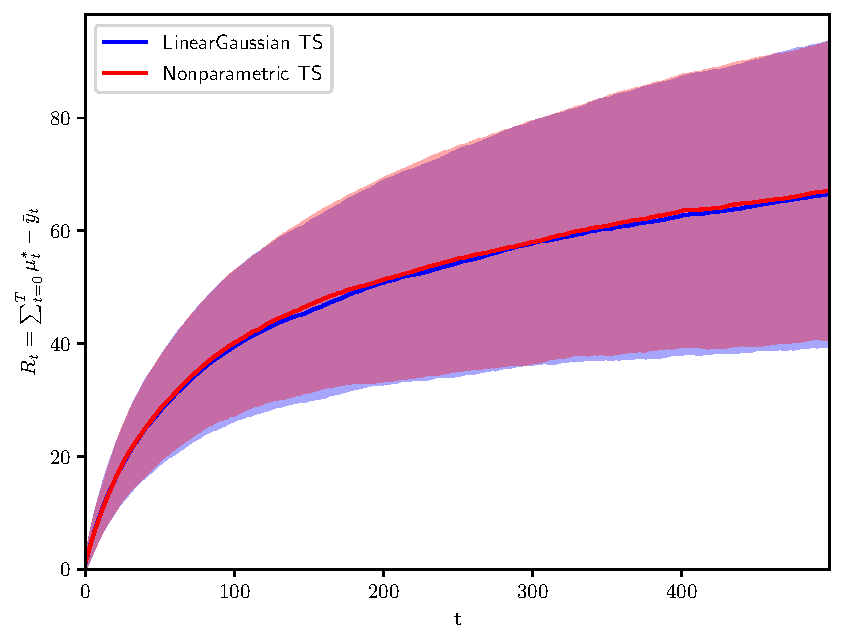
\includegraphics[width=\textwidth]{./figs/linearGaussian/cumregret_A5_-1_-1_-05_-05_0_0_05_05_1_1_1_1_1_1_1}
		\vspace*{-5ex}
		\caption{$|\mathcal{A}|=5, \theta_{0,i}=-1$,\\ \hspace*{0.3cm} $\theta_{1,i}=-0.5$, $\theta_{2,i}=0$,\\ \hspace*{0.3cm} $\theta_{3,i}=0.5, \theta_{4,i}=1$.}
		\label{fig:linear_gaussian_A5_05}
	\end{subfigure}
	\begin{subfigure}[b]{0.32\textwidth}
		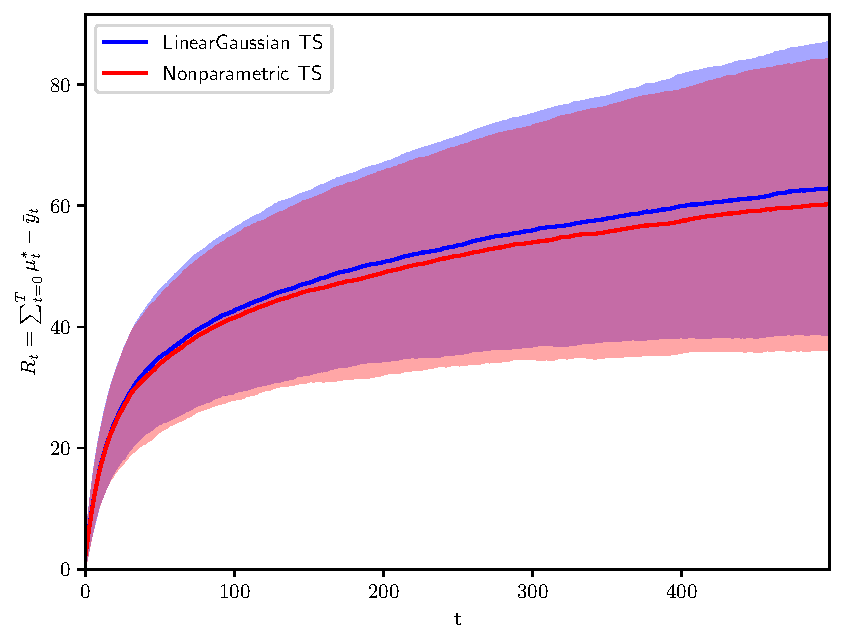
\includegraphics[width=\textwidth]{./figs/linearGaussian/cumregret_A5_-2_-2_-1_-1_0_0_1_1_2_2_1_1_1_1_1}
		\vspace*{-5ex}
		\caption{$|\mathcal{A}|=5, \theta_{0,i}=-2$,\\ \hspace*{0.3cm} $\theta_{1,i}=-1$, $\theta_{2,i}=0$,\\ \hspace*{0.3cm} $\theta_{3,i}=1, \theta_{4,i}=2$.}
		\label{fig:linear_gaussian_A5_1}
	\end{subfigure}
	%\vspace*{-2ex}
	\caption{Mean cumulative regret (and standard deviation shown as shaded region) for $R=1000$ realizations of different $\A=\{2,3,4,5\}$ armed contextual linear Gaussian bandits, with $\sigma_a^2=1 \forall a$.}
	\label{fig:linear_gaussian_oracle}
	%\vspace*{-4ex}
\end{figure*}

We showcase the flexibility of our proposed method in the contextual linear Gaussian MAB setting first, where we can readily compare its performance to a well studied \texttt{Oracle TS}: \ie the linear Gaussian Thompson sampling in~\cite{ip-Agrawal2013a}.
In this set-up, \texttt{LinearGaussian TS} correctly assumes the true underlying contextual linear Gaussian model $Y_{t,a}\sim \N{Y|x_t^\top\theta_a, \sigma_a^2}$, and can compute posterior updates in closed form. 

In Figure~\ref{fig:linear_gaussian_oracle}, we show the mean cumulative regret of various parameterizations of multi-armed ($\A=\{2,3,4,5\}$) contextual linear Gaussian bandits, with two-dimensional contexts randomly drawn from a uniform distribution, \ie $x_{i,t}\sim\U{0,1}$, $i\in\{0,1\}$, $t\in \Natural$.

The proposed \texttt{Nonparametric TS} attains cumulative regret comparable to that of \texttt{LinearGaussian TS}. 
That is, the proposed method matches the performance of the analytical linear Gaussian posterior Thompson sampling, even as it estimates the true form of the underlying reward function.

The proposed nonparametric Thompson sampling is almost as good as the analytical alternative when there is no model mismatch, as in this setting: the per-arm nonparametric posterior density quickly converges to the true unknown distribution, incurring in minimal additional regret when compared to the analytical posterior based \texttt{Oracle TS} alternative.

% Not-exponential contextual bandits
% !TEX root = main.tex
\subsubsection{Contextual bandits not in the exponential family: Oracle TS}
\label{sssec:evaluation_mixture_scenarios_oracle}

We further scrutinize Algorithm~\ref{alg:nonparametric_ts} by comparing it to \texttt{Oracle TS} algorithms for \texttt{Scenarios A}, \texttt{B}, \texttt{C} and \texttt{D}.
We implement separate \texttt{Oracle TS} algorithms for each scenario, via a Dirichlet prior distribution that has knowledge of the true underlying dimensionality $K_a$ per-arm.

This approach is similar to~\cite{ip-Urteaga2018}, where mixtures of Gaussian distributions model per-arm reward functions.
To provide a fair comparison to our proposed method, and instead of the variational inference-based original approach of~\citet{ip-Urteaga2018}, we implement a Gibbs sampler as described in Section~\ref{sec:proposed_method} where for each \texttt{Oracle TS}, the correct $K_a$ per-scenario is known (instead of the Dirichlet process prior assumed by \texttt{Nonparametric TS}).

We compare the performance of our proposed nonparametric Thompson sampling to that of each per-scenario \texttt{Oracle TS} in Figure~\ref{fig:mixture_scenarios_oracle}.
The proposed nonparametric Thompson sampling provides satisfactory performance across all studied scenarios, when compared to an unrealistic \texttt{Oracle TS} that knows the true number of underlying mixtures of the problem it is targeted to.

% Nonparametric and Oracle in scenarios
\begin{figure*}[!h]
	\centering
	\begin{subfigure}[c]{0.45\textwidth}
		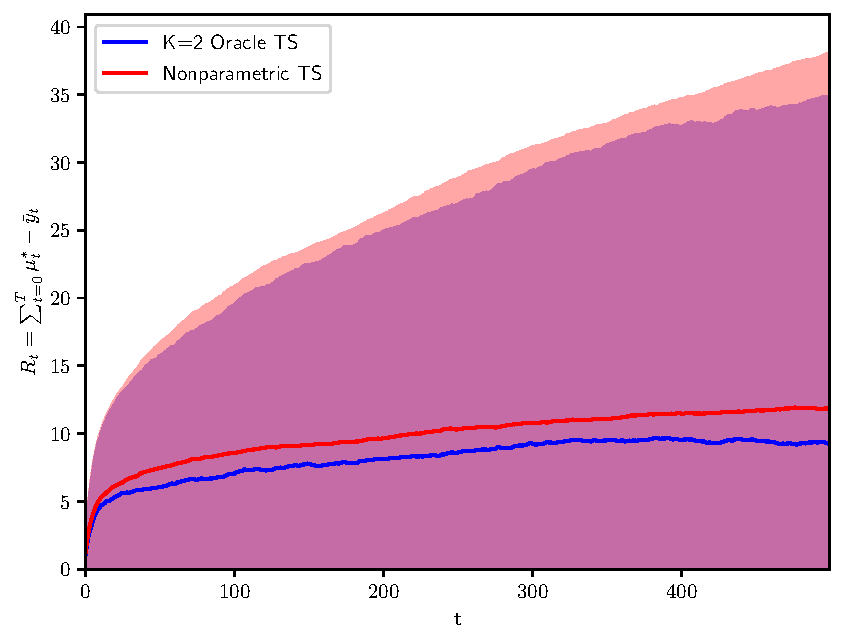
\includegraphics[width=\textwidth]{./figs/linearGaussianMixture/easy/cumregret_R3742.pdf}
		\vspace*{-5ex}
		\caption{\texttt{Scenario A}.}
		\label{fig:scenario_A_oracle}
	\end{subfigure}
	\begin{subfigure}[c]{0.45\textwidth}
		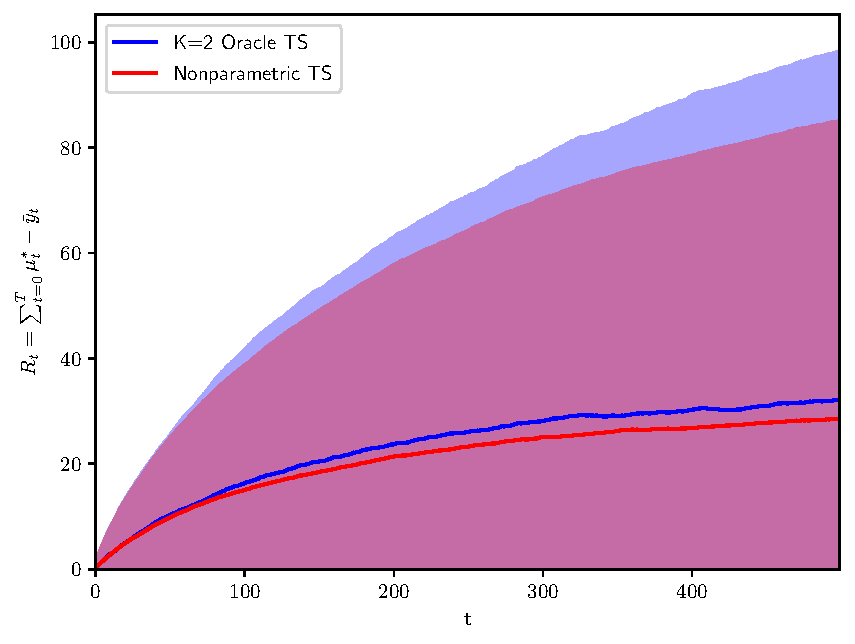
\includegraphics[width=\textwidth]{./figs/linearGaussianMixture/hard/cumregret_R3629.pdf}
		\vspace*{-5ex}
		\caption{\texttt{Scenario B}.}
		\label{fig:scenario_B_oracle}
	\end{subfigure}
	
	\begin{subfigure}[c]{0.45\textwidth}
		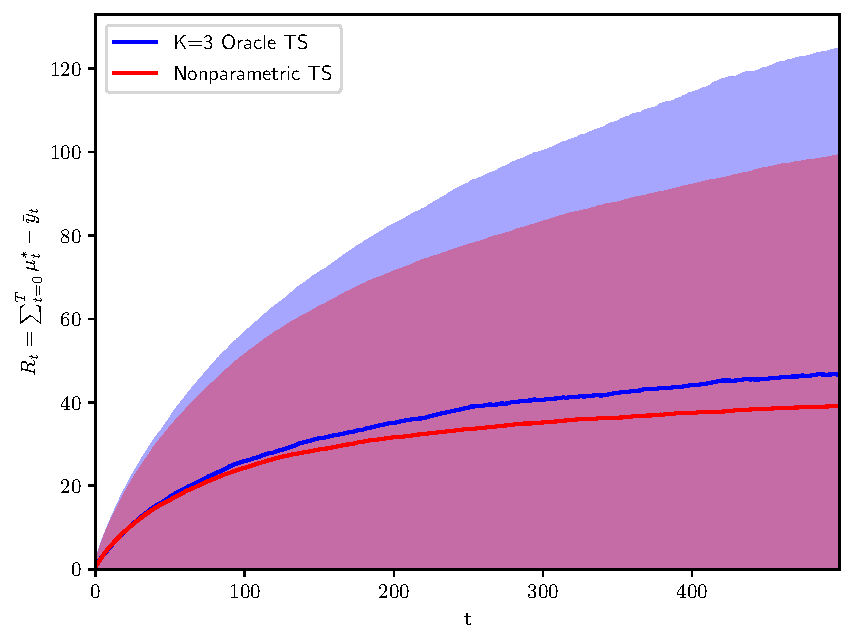
\includegraphics[width=\textwidth]{./figs/linearGaussianMixture/unbalanced/cumregret_R3641.pdf}
		\vspace*{-5ex}
		\caption{\texttt{Scenario C}.}
		\label{fig:scenario_C_oracle}
	\end{subfigure}
	\begin{subfigure}[c]{0.45\textwidth}
		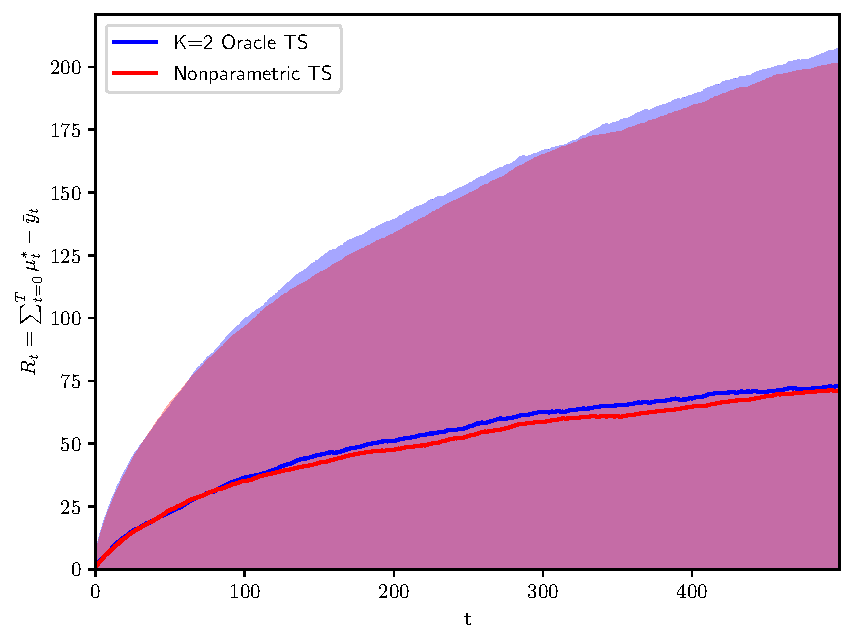
\includegraphics[width=\textwidth]{./figs/linearGaussianMixture/heavy/cumregret_R3250}
		\vspace*{-5ex}
		\caption{\texttt{Scenario D}.}
		\label{fig:scenario_D_oracle}
	\end{subfigure}
	\vspace*{-2ex}
	\caption{Mean regret (standard deviation shown as shaded region) for $R=3000$ realizations of the proposed and \texttt{Oracle TS} methods.}
	\label{fig:mixture_scenarios_oracle}
	\vspace*{-2ex}
\end{figure*}

The \texttt{Nonparametric TS} fits the underlying reward function accurately in all cases, attaining comparable regret in all scenarios.
We emphasize that the \texttt{Nonparametric TS} method does not demand any per-scenario hyperparameter tuning, and avoids model misspecification: \ie the same algorithm is used for all scenarios, while scenario specific \texttt{Oracle TS} methods are required.

These results demonstrate the competitive advantage of Bayesian nonparametrics to adjust the complexity of the reward model to the sequentially observed bandit data.
The proposed nonparametric generative modeling provides per-arm reward understanding (by plotting or computing figures of merit from these distributions), as the learned per-arm posteriors converge to the true posteriors.
We note that nonparametric posterior density convergence does not imply that it is consistent in $K$ ---on data from a finite mixture, nonparametric posteriors do not necessarily concentrate at the true number of components~\citep{j-Miller2014}. Nevertheless, we argue that density convergence suffices in the bandit setting.

% Misspecification, moved here for a better placement in the article
\begin{figure}[!h]
	\centering
	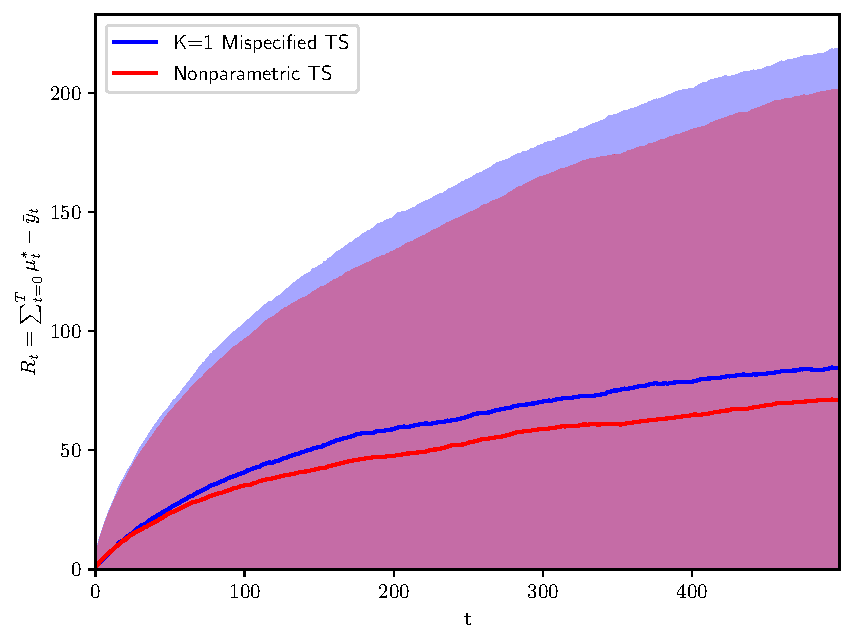
\includegraphics[width=0.75\textwidth]{./figs/linearGaussianMixture/heavy/cumregret_R3250_mispecified}
	\vspace*{-5ex}
	\caption{Mean regret (standard deviation shown as shaded region) for $R=3000$ realizations of the proposed and \texttt{Oracle TS} methods in \texttt{Scenario D} under model misspecification.}
	\label{fig:mixture_scenarios_misspecified}
	\vspace*{-2ex}
\end{figure}

We further highlight the built-in flexibility of the proposed nonparametric method by showing in Figure~\ref{fig:mixture_scenarios_misspecified} how Thompson sampling with a mispecified model (\ie fitting a unimodal Gaussian distribution to the heavy-tailed \texttt{Scenario D}) suffers in comparison to the proposed nonparametric method: a \%18 cumulative regret reduction is attained by \texttt{Nonparametric TS}.
With this, we reiterate the robustness and generality of our proposed nonparametric method in avoiding model-misspecification, a significant advantage for real-life bandit settings.

We conclude by emphasizing that the proposed \texttt{Nonparametric TS} avoids stringent case-by-case model assumptions for each specific MAB setting, yet attains competitive regret when faced with distinct, complex MAB reward distributions: the same algorithm (with no hyperparameter tuning) is run for contextual Gaussian bandits and other complex (not in the exponential family) multi-armed bandits.